%!TEX root=../document.tex

\section{Aufgabenstellung 1.UE}
Nachbau eines Garagentor mittles eine Induktionsplatte. Beim simulierten Aufgehen des Tores soll eine rote Lampe leuchten. Es gibt einen Motor mit zwei Eingängen (1/EIN und 0/Aus) und (DIR 1/nach oben und 0/nach unten). Außerdem soll das Garagentor auch eine Lichtschranke besitzen welche \textbf{0 fuer unterbrochen} und \textbf{1 fuer nicht unterbrochen} sendet. Ein Endschalter sollte zur Sichherheit auch vorhanden sein (\textbf{1 Kontakt sonst 0})
\textbf{Der Ablauf sollte dann folgendermaßen Aussehen:}
\begin{itemize}
	\item Auto da -> Tor aufgehen
	\item Tor bewegt sich -> rot Lampe an
	\item Tor offen -> gruene Lampe
	\item Tor bleibt offen wenn Lichtschranke unterbrochen
	\item Tor schließt wenn Lichtschranke mindestens 40 sec nicht mehr unterbrochen wurde.
\end{itemize}

\begin{figure}[!h]
	\begin{center}
		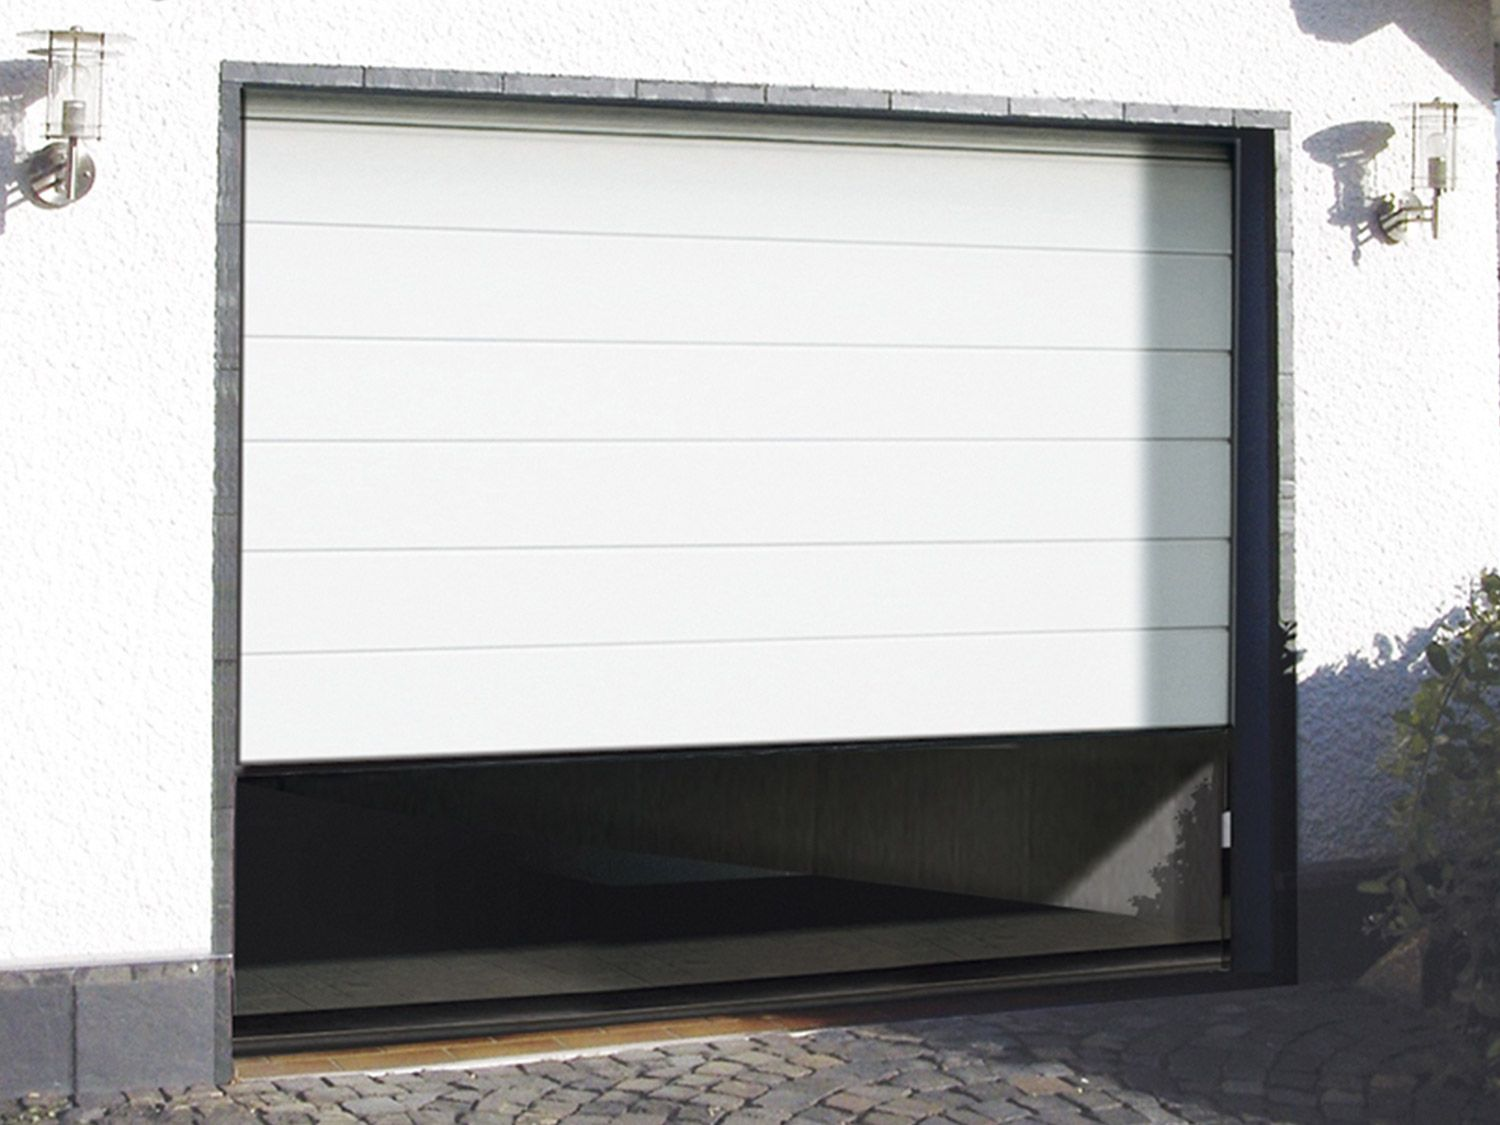
\includegraphics[width=0.5\linewidth]{images/garagentor}
		\caption{Abbildung eines elektronischen Garagentors}
		\label{garage}
	\end{center}
\end{figure}
\newpage

\section{Ergebnisse 1.UE}
Um die benoetigte Schaltung zu entwickeln benoetigt man zunächst eine Wahrheitstbelle mit allen Ein- und Ausgaengen und ihre moeglichen Varitationen der Werte. 


\begin{table}[!h]
	\centering
	\caption{Tabelle der richtige Kombinationen}
	\label{UE1}
	\begin{tabular}{l|l|l|l|l|l}
		\cline{2-5}
		& \textbf{A}          & \textbf{A}          & \textbf{As}         & \textbf{As}         & \textbf{}                        \\ \hline
		\multicolumn{1}{|l|}{\textbf{C}}  & \textit{\textbf{1}} & 0                   & \textit{\textbf{1}} & \textit{\textbf{1}} & \multicolumn{1}{l|}{\textbf{D}}  \\ \hline
		\multicolumn{1}{|l|}{\textbf{C}}  & \textit{\textbf{1}} & \textit{\textbf{1}} & \textit{\textbf{1}} & 0                   & \multicolumn{1}{l|}{\textbf{Ds}} \\ \hline
		\multicolumn{1}{|l|}{\textbf{Cs}} & \textit{\textbf{1}} & 0                   & \textit{\textbf{1}} & \textit{\textbf{1}} & \multicolumn{1}{l|}{\textbf{Ds}} \\ \hline
		\multicolumn{1}{|l|}{\textbf{Cs}} & \textit{\textbf{1}} & 0                   & \textit{\textbf{1}} & \textit{\textbf{1}} & \multicolumn{1}{l|}{\textbf{D}}  \\ \hline
		& \textbf{B}          & \textbf{Bs}         & \textbf{Bs}         & \textbf{B}          & \textbf{}                        \\ \cline{2-5}
	\end{tabular}
\end{table}

\textbf{Aus dieser Tabelle ergeben sich folgende Muster:}
\begin{itemize}
	\item (A UND B UND C UND D) UND (A UND B UND Cs UND D) UND \newline (As UND B UND C UND D) UND (As UND B UND Cs UND D)
	\item (As UND Cs) ODER (Cs UND B) ODER (C UND Cs UND D UND Ds) ODER \newline (C UND Cs UND D UND Ds) UND (B UND D)
\end{itemize}
\textbf{Herausgehoben kommt man zu folgendem Ergebnis:}
\begin{center}
	\textbf{Cs UND (A ODER B ODER D UND [(C UND DS) ODER B])}
\end{center}
\newpage
\section{Aufgabenstellung 2.UE}
Die Aufgabe der 2. Unterrichtseinheit bestand darin, eine Ampelsteuerung auf einem Raspberry Pie entwickelt durch CodeSys auszuführen. Hierbei mussten ein paar Vorbereitungen getroffen werden. Zunaechst die Installation der Entwicklungsumgebung CodeSys V3.5 SP9. Danach musste noch ein zusätzliches Paket fuer den Raspberry Pie installiert beziehungsweise heruntergeladen werden. (CODESYS Control for Raspberry PI 3.5.9.40)
Nach der erfolgreichen Installation und dem \textbf{Anlegen eines neuen Projektes:}


\begin{figure}[!h]
	\begin{center}
		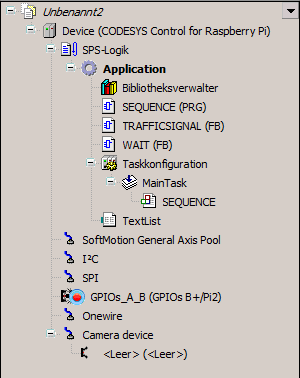
\includegraphics[width=0.5\linewidth]{images/projektstruktur}
		\caption{Aufbau eines Projektes}
		\label{aufbauprojekt}
	\end{center}
\end{figure}
\newpage
Danach muessen die GPIO-Pins richtig gesetzt werden, sprich INPUT/OUTPUT:
\begin{figure}[!h]
	\begin{center}
		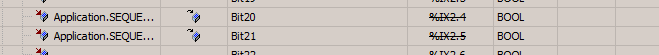
\includegraphics[width=0.8\linewidth]{images/input}
		\caption{Auf Input gesetzten GPIO-Pins}
		\label{aufbauprojekt}
	\end{center}
\end{figure}

\begin{figure}[!h]
	\begin{center}
		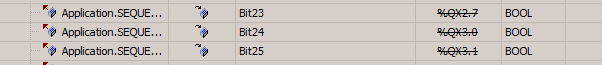
\includegraphics[width=0.8\linewidth]{images/output}
		\caption{Auf Output gesetzten GPIO-Pins}
		\label{aufbauprojekt}
	\end{center}
\end{figure}

\section{Ergebnisse 2.UE}
Bevor man nun mit der Entwicklung des Codes starten kann muss man noch die Pins noch \textbf{gemappt} werden. Dies passiert in der selben Tabelle, wie auf den oberen Abbildungen gezeigt.

\begin{lstlisting}[style=Java, caption=SEQUENCE PRG]
PROGRAM SEQUENCE
VAR_INPUT
START : BOOL;
SCHALTER1 : BOOL;
SCHALTER2 : BOOL;
END_VAR
VAR_OUTPUT
TRAFFICSIGNAL_RED : BOOL;
TRAFFICSIGNAL_YELLOW: BOOL;
TRAFFICSIGNAL_GREEN : BOOL;
END_VAR
\end{lstlisting}

\begin{figure}[!h]
	\begin{center}
		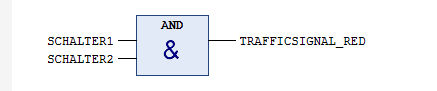
\includegraphics[width=0.8\linewidth]{images/sequence}
		\caption{Abbildung des SEQUENCE PRG}
		\label{aufbauprojekt}
	\end{center}
\end{figure}

\begin{lstlisting}[style=Java, caption=TRAFFICSIGNAL FB]
FUNCTION_BLOCK TRAFFICSIGNAL
VAR_INPUT
STATUS : INT;
END_VAR
VAR_OUTPUT
GREEN : BOOL;
YELLOW : BOOL;
RED : BOOL;
random : BOOL;
END_VAR
\end{lstlisting}

\begin{figure}[!h]
	\begin{center}
		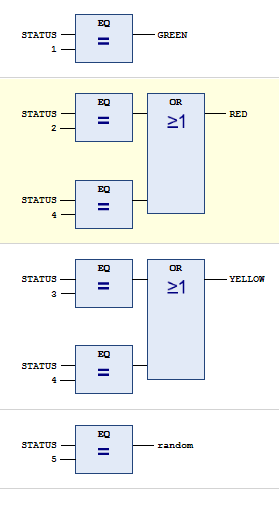
\includegraphics[width=0.4\linewidth]{images/fb}
		\caption{Abbildung der Funktionsbloecke}
		\label{aufbauprojekt}
	\end{center}
\end{figure}

\newpage


\begin{lstlisting}[style=Java, caption=TRAFFICSIGNAL FB]
FUNCTION_BLOCK WAIT
VAR_INPUT
TIME_IN : TIME;
END_VAR
VAR_OUTPUT
OK:BOOL := FALSE;
END_VAR
VAR ZAB:TP;
END_VAR
\end{lstlisting}

